\documentclass[../index.tex]{subfiles}

\begin{document}

Мало кто знает, что история динамического языка началась задолго до появления автоматизированной системы <<Лицо Друга>>. Первые зачатки динамических форм родились в славном городе Ростов, более 10 лет назад.


Кирилл Борисович Кривошеев, создатель динамического языка,  в те времена работал начальником отдела внедрения и сопровождения автоматизированных систем Юго-Западного территориального банка ПАО Сбербанк. Работы было много и, несмотря на всю самоотверженность и трудолюбие сотрудников, на отдел постоянно поступали жалобы. И причина тому была воистину «сбербанковская»: с утра и до позднего вечера сотрудники разгребали сотни заявок от пользователей на просьбы разблокироваться в каких-либо системах. На одного сотрудника в день могло назначаться более 200 заявок. Звонили пользователи, просили разблокировать их учётные записи, по звонку регистрировались запросы, которые затем передавались в другие подразделения. Далее искали заявителя в базе и выясняли причину проблемы. А причины могли быть самые нелепые, например, пользователь вместо логина упорно вбивал какую-нибудь хрень.


Вся эта ситуация будоражила сознание Кирилла, а вокруг никто не желал пошевелить и пальцем, чтобы как-то улучшить процесс, зато ежедневных жалоб и нытья было вагон и маленькая тележка.
И тут Кирилл начал задумываться о способах автоматизации процессов.

\section{Вижу цель не вижу препятствий}

В 2010 году Кирилл Борисович перешел на должность заместителя директора управления внедрения и сопровождения Юго-Западного территориального банка. После вступления в должность, Кирилл стал отвечать за всю автоматизацию банка, и, помимо отдела внедрения и сопровождения, под его руководством оказалась диспетчерская служба.

Теперь он наблюдал за еще большим количеством сотрудников, страдающих от скучных рутинных процессов.

Понимая, что если не он, то никто, Кирилл принялся за написание программы по оптимизации процесса разблокировки учетных записей. При этом стоит отметить, что на тот момент Кирилл Борисович толком не знал ни одного языка программирования, не считая языка PL+ -- помеси SQL и объектно-ориентированного подхода, на котором были написаны многие автоматизированные системы.

Писать на PL+ было не вариант, но Кирилла это не остановило. “Гугл в помощь” -- и вот наш герой уже шпарит свою первую программу на свежевыученном языке программирования C\#. Всего было 25 программ для 25-ти автоматизированных систем. И эти 25 программ могли экономить для каждого пользователя примерно час жизни, которые ранее уходили на получение доступа, подачу заявки и ожидание в очереди на исполнение. Программа же справлялась с задачей всего за 30 секунд!

“Зашибись!” — подумал Кирилл, и пошел продавать идею заместителю председателя банка. И тут барьеры на пути к цели вновь дали о себе знать. Задумка была отклонена, а вместо нее была дана рекомендация нанять побольше людей в контактные центры и научить их нормально работать…

Вера в банковскую утопию, где сотрудники не должны были бы страдать от рутинных бессмысленных процессов, все же не покидала Кирилла. И он решил совершить ход конем. Удачным стечением обстоятельств явилось то, что в том году в банке по всей стране происходило довольно значимое событие: Программа глобального внедрения производственной системы в Сбербанке под руководством самого Германа Грефа. Данная система была вдохновлена лучшим практиками компании Тойота. Именно благодаря ей и по сей день в банке проводится Гемба, -- процесс, когда начальник сам становится за станок, чтобы понимать проблемы изнутри, испытывая их на личном опыте.

Вместе с Гембой пришло поручение сверху оптимизировать всё, что только можно оптимизировать. Например, был процесс связанный с чековой книжкой: после каждой операции, в соответствии с нормативными документами нужно было распечатать чековую книжку, поставить печать, зарегистрировать ее и т.д. На*ера?! Клиент этого не хочет, потребности у него такой точно нет. А сотрудник тратил довольно много времени на эти бессмысленные процессы.  И вот, в рамках оптимизации, отменили сначала печати, а потом и вовсе чековые книжки.

Кириллу, как заместителю директора, также пришло поручение оптимизировать процессы внутри отделов. И тут, не растерявшись, Кирилл Борисович решил повторно презентовать свою идею, но только теперь уже напрямую в центральный аппарат. Идея была принята. Так появилась на свет программа B@nk Helper -- программа, которая помогала пользователям быстро получить доступ в необходимую систему.

\begin{figure}[h]
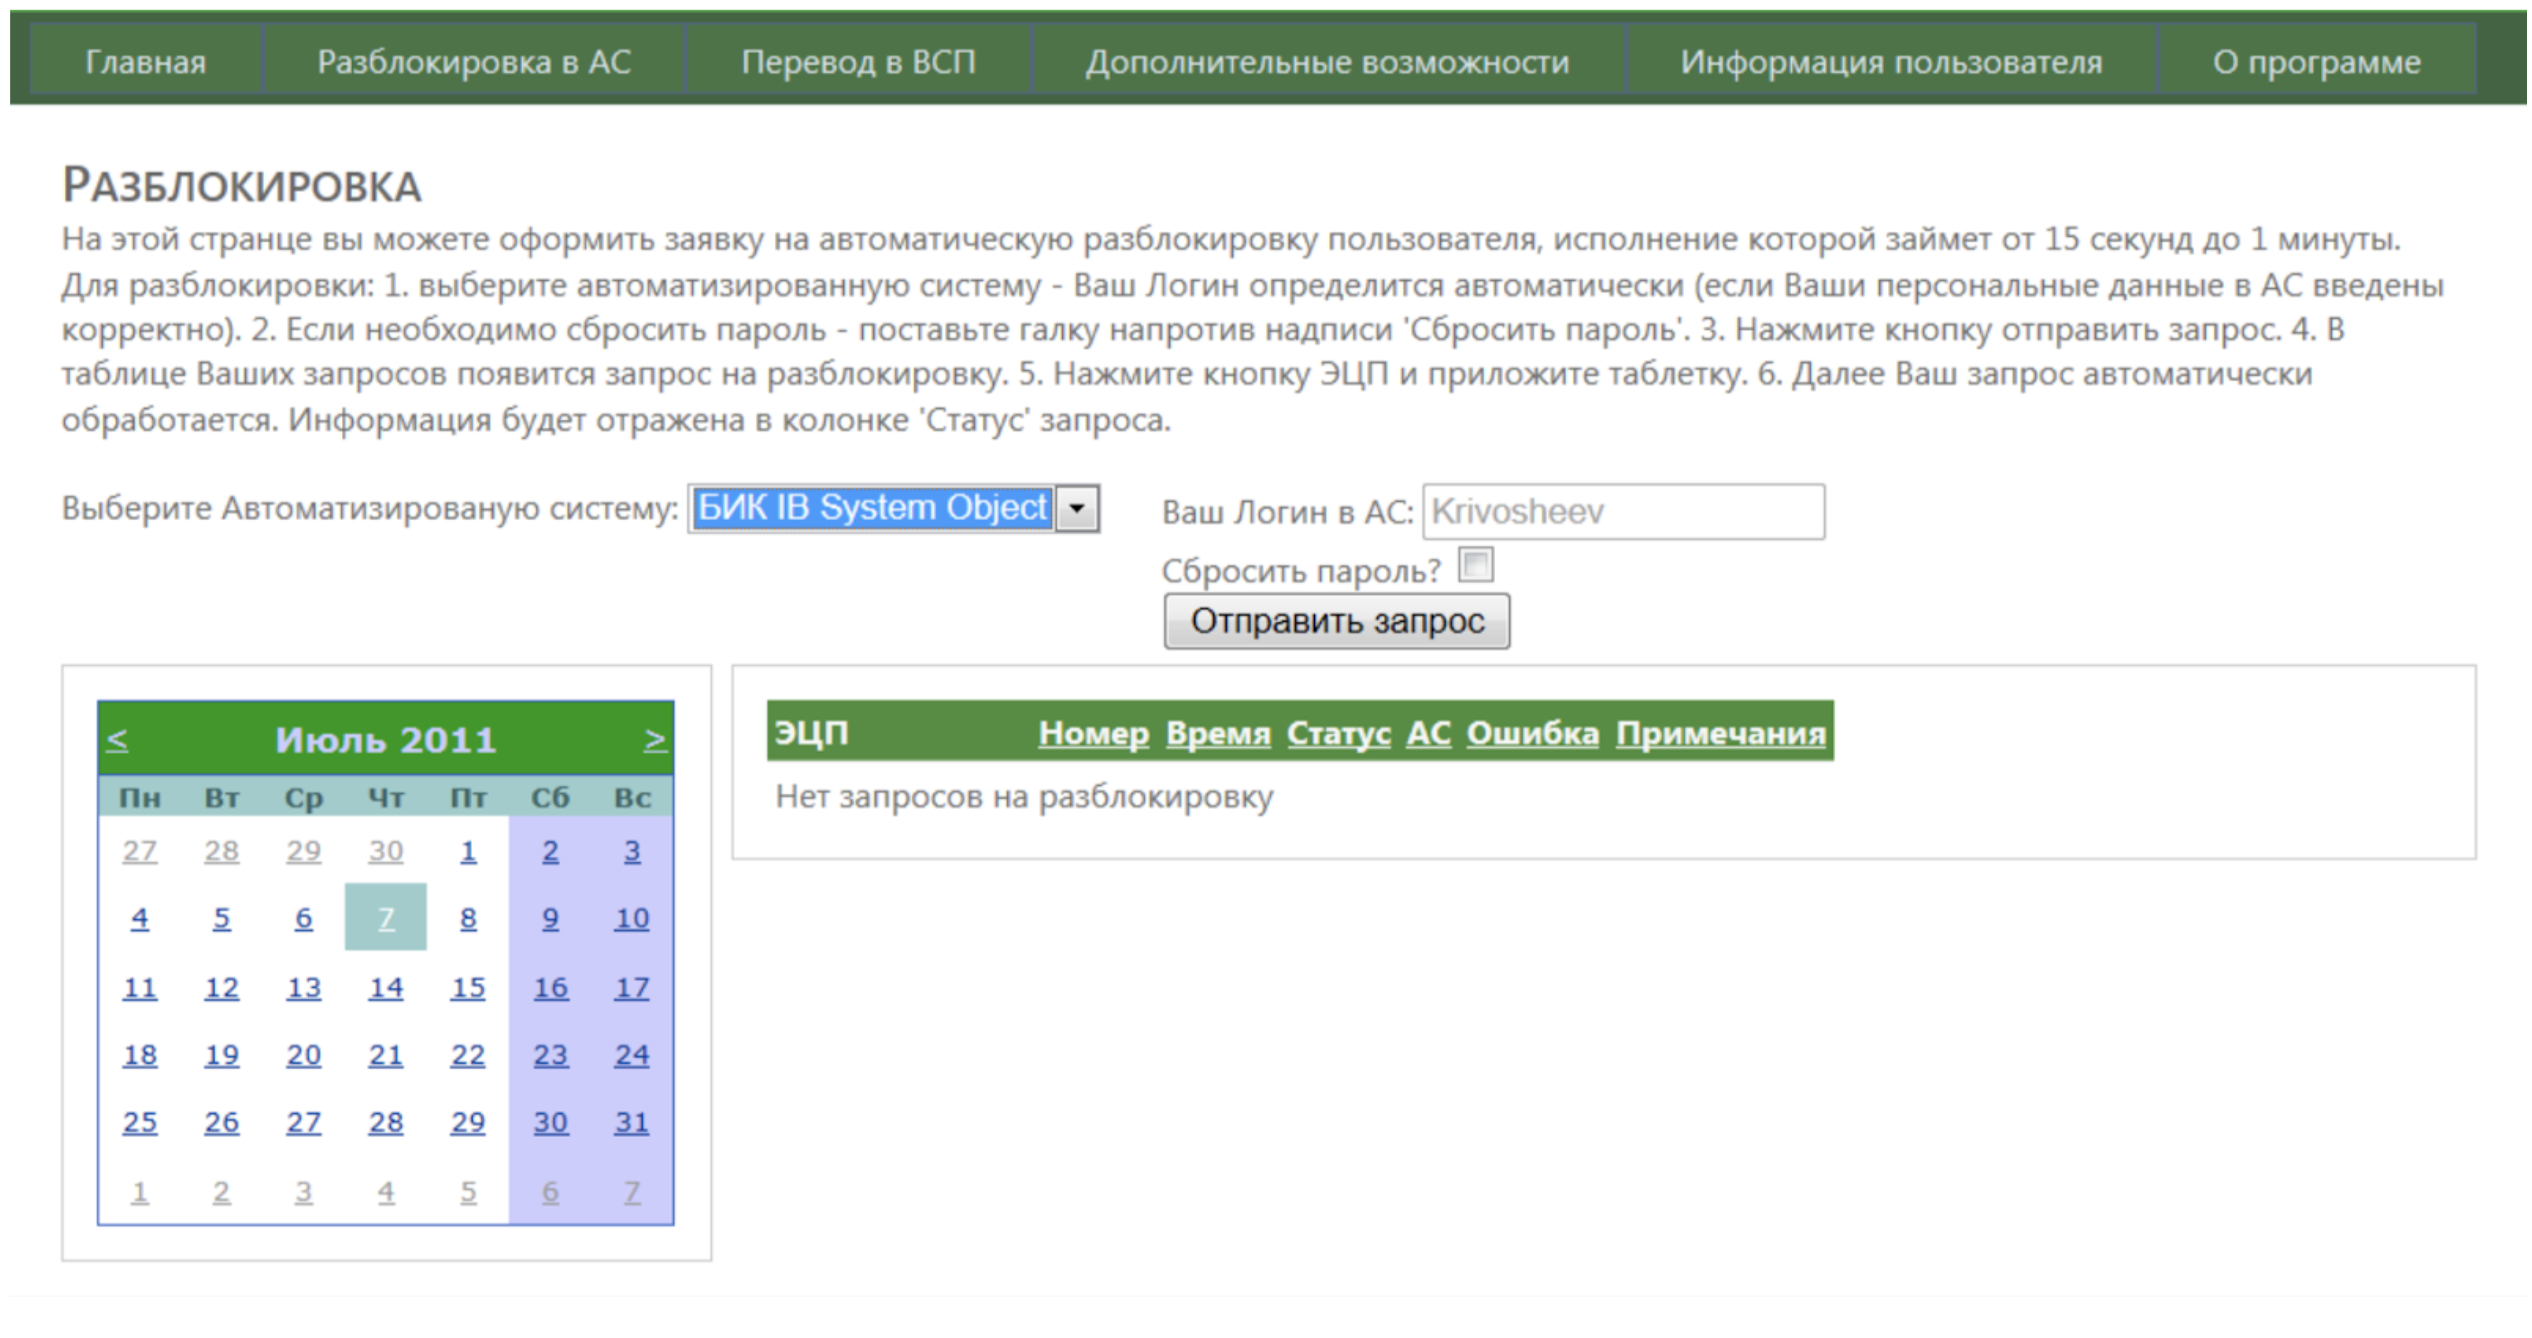
\includegraphics[width=0.9\textwidth]{bankhelper}
\centering
\end{figure}

\section{Первый успех и рождение динамических форм}

\begin{figure}[H]
	\includegraphics[width=0.7\textwidth]{bh_passport}
	\centering
\end{figure}

Итак, программа B@nk Helper была запущена и представлена всем заведующим филиалов банка в городе Ростов и, чтобы вы понимали, это 80 женщин (!).
После презентации к Кириллу подошел директор, и сказал:
“Еще никогда в жизни я не видел такого количества одновременно оргазмирующих женщин!”.

И это было только начало. B@nk Helper сразу полюбился сотрудникам банка, но, как говорится, к хорошему привыкаешь быстро. Вскоре начали поступать запросы на дополнительные изменения в программе, например, добавить галочку или списочек. И Кирилл, конечно же,  совершенствовал B@nk Helper. Но изменения в системе давались не так просто, ведь приходилось вносить их в каждой форме для 25 однотипных автоматизированных систем. Так появился еще один процесс, который было необходимо оптимизировать.

Кирилл Борисович начал думать над тем, как унифицировать процессы, как избавить себя от необходимости кодить каждый раз и не тратить на это уйму времени, а иметь возможность через простые настройки настраивать формы как надо. И именно такой способ настройки форм и придумал Кирилл. Способ, при котором не нужно было проводить ПСИ (приемо-сдаточные испытания), отдельно выводить функционал в промышленную эксплуатацию.  Формы программы можно было настроить в любой момент так, как необходимо.

Запросы не прекращались, появилась потребность при изменении одного поля ввода, в зависимости от введённых в него данных автоматически подгружать другое поле ввода. Кирилл придумал как справиться и с этой задачей. Эти формы и стали первым прототипом динамических форм, таких, какими мы знаем их сейчас.

Таким образом B@nk Helper стал прекрасным решением как для пользователей, так и для разработчиков. А Кирилл даже получил почетное звание “Инноватор Года”, которое записано в его паспорте участника  корпоративной системы работы с инновациями. Этот паспорт по сей день  бережно хранится шкафчике в кабинете Кирилла Борисовича.

\begin{figure}[H]
	\includegraphics[width=0.7\textwidth]{bh_passport_2}
	\centering
\end{figure}

В тоже время, помимо наград и всеобщего признания  Кириллу Борисовичу поступило официальное предложение о переезде в Москву для тиражирования  системы B@nk Helper во все территориальные банки.

\section{80 счастливых женщин — не предел}

«Что за гадюшник ты снял?» — примерно с таких слов супруги началась жизнь Кирилла Борисовича в Москве. Но не переживайте, в итоге семья осталась довольна, гадюшник оказался прекрасным уютным гнездышком, да еще и по соседству с давним ростовским другом Кирилла.

В Москве Кирилл Борисович начал работу в одном из самых прогрессивных подразделений банка — Сбербанк Технологии. Его должность называлась руководитель разработки, но по правде говоря руководил он больше сам собой.  Один на один с задачей растиражировать B@nk Helper, он вдохновленно начал работу. На тот момент существовало 17 территориальных банков, Кирилл прописал необходимые инструкции, назначил ответственных в банках и запустил процесс тиражирования продукта. B@nk Helper был встречен сотрудниками с овациями, о нем писали в газете, и те 80 оргазмирующих женщин — только маленькая часть  довольных и удовлетворенных отличным сервисом сотрудников.

По самым минимальным подсчетам B@nk Helper сэкономил банку более 40 миллионов рублей в год. 

Дальше — больше! Следующий этап развития B@nk Helper случился в связи с приходом задачи от Центров Сопровождения Клиентских Операций. У них была потребность обмениваться информацией между центрами в разных территориальных банках. На тот момент B@nk Helper имел отдельные сервера на каждой территории, но после доработки, можно было отправлять запросы из одного региона в другой.

\section{Портал самообслуживания}

После оглушительного успеха  B@nk Helper пришло время заняться следующим проектом — порталом самообслуживания. Это еще один портал, но теперь для сервис-менеджера. 
В отличии от B@nk Helper, портал самообслуживания был написан на GWT — фреймворке, на котором в будущем будет написано Лицо Друга 1.0. 

Именно на портале самообслуживания и родились первые полноценные шаблоны с динамическим языком. Для чего это было сделано: раньше у пользователя было одно окошко, где он мог оставить информацию о своей проблеме в свободном формате. Для  исполнителя это становилось каждодневным вызовом — провести лексический анализ потока сознания пользователя и вычленить информацию, необходимую для закрытия задачи.

\begin{figure}[H]
	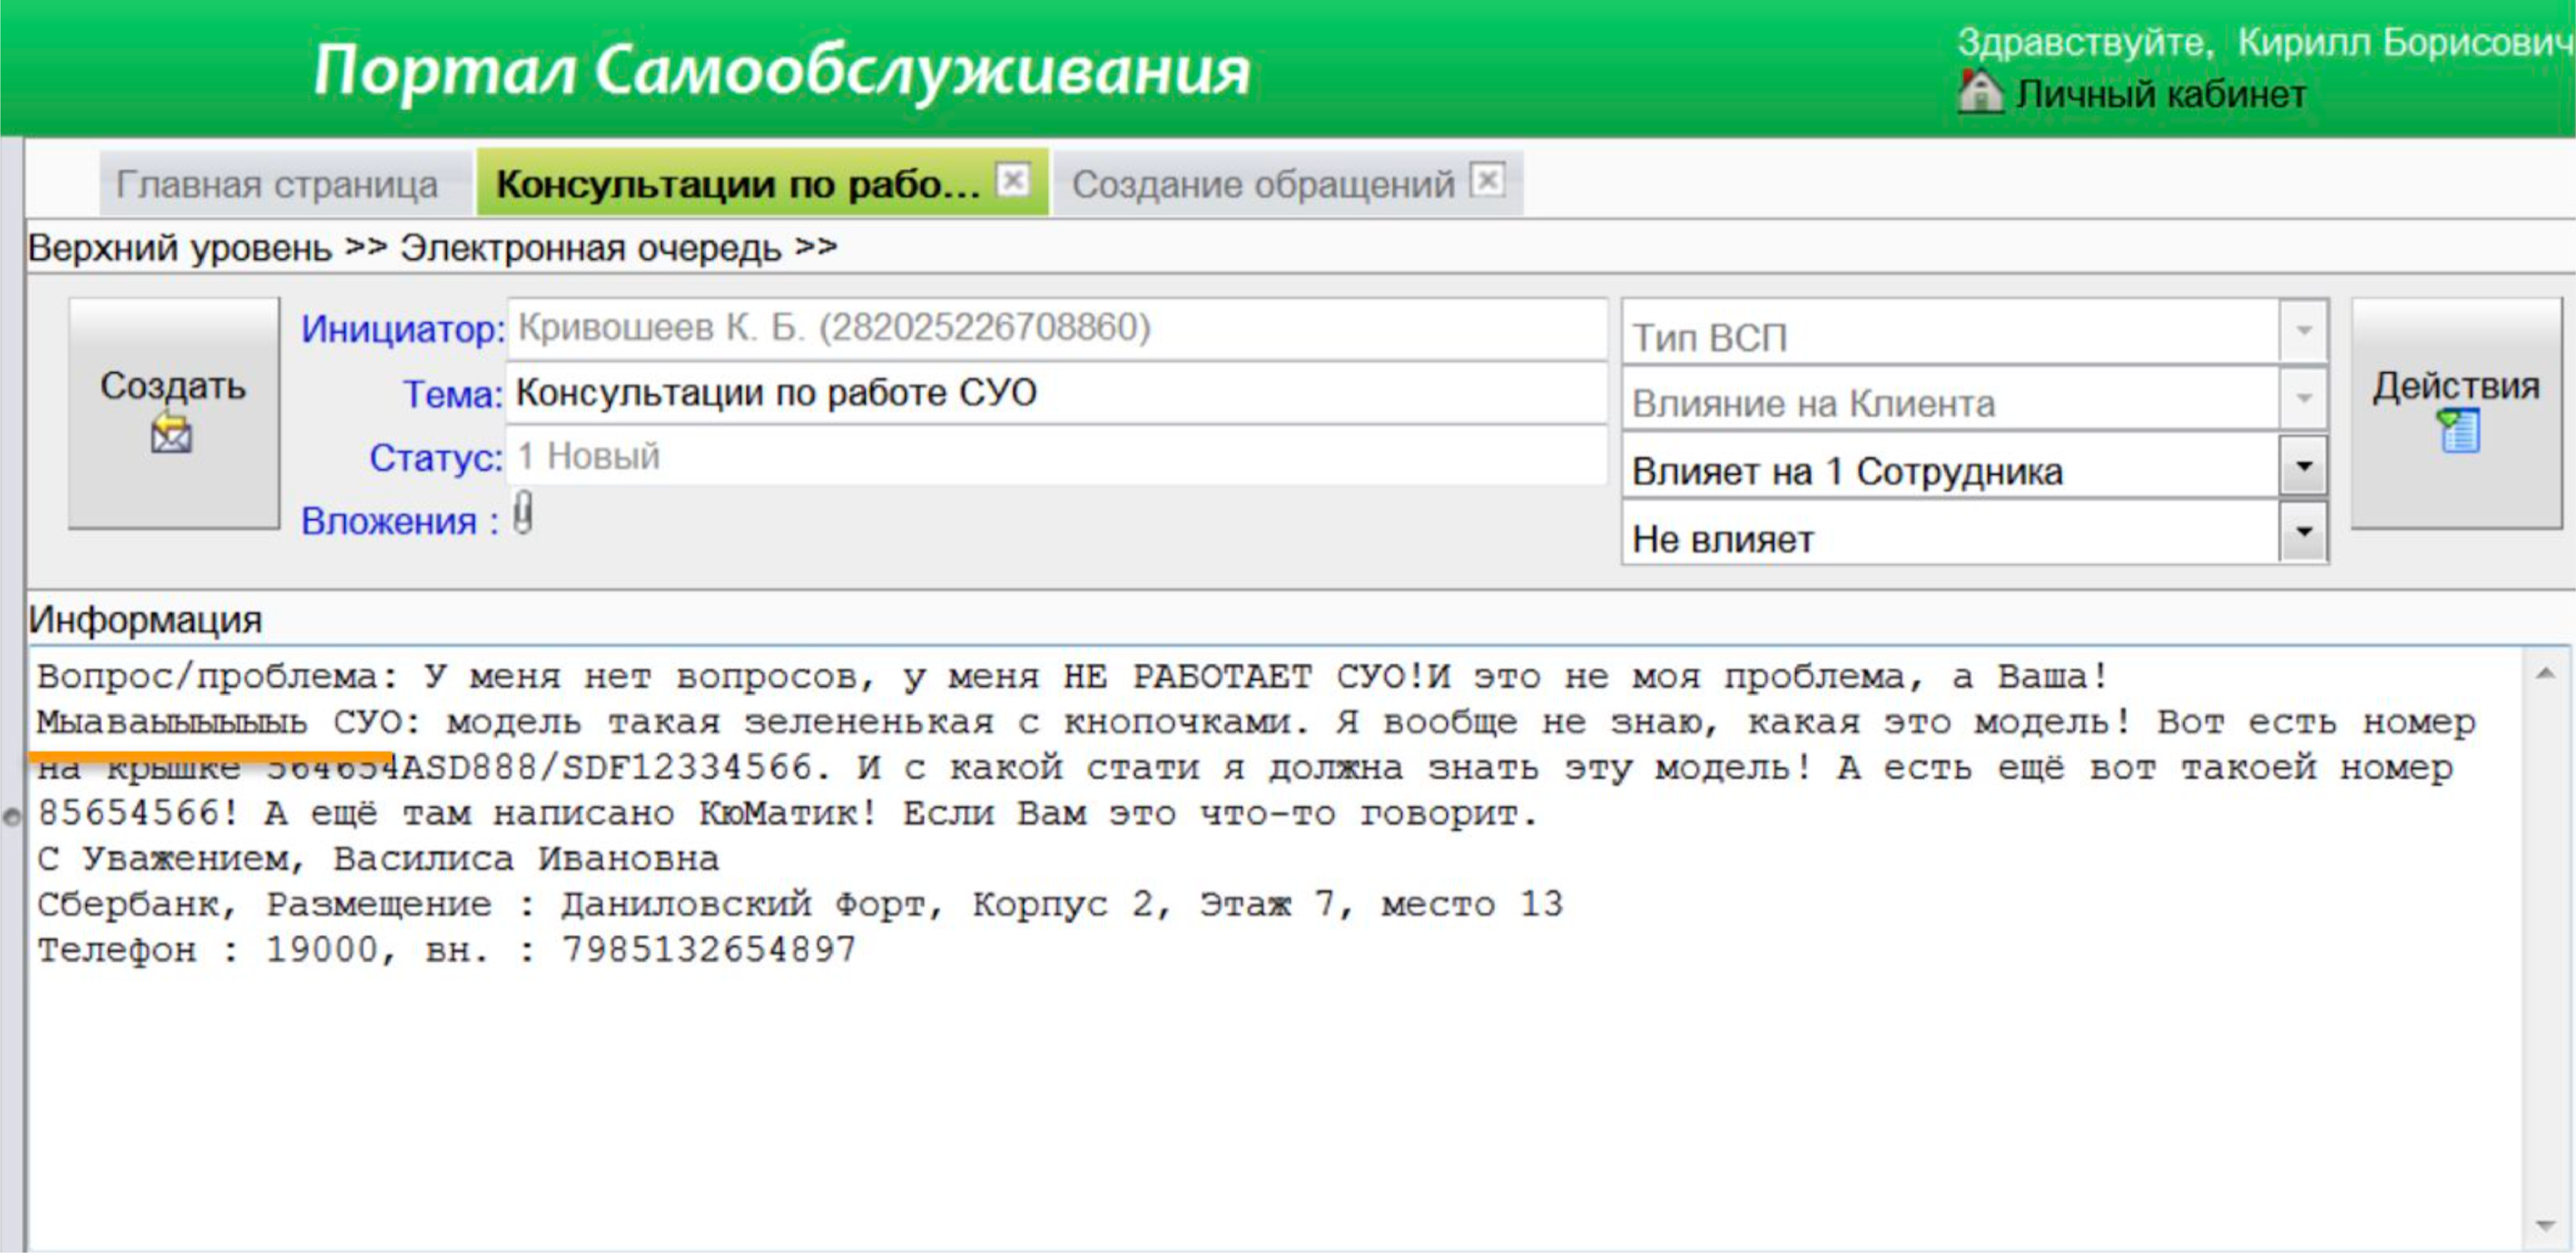
\includegraphics[width=1\textwidth]{portal_1}
	\centering
\end{figure}

После внедрения динамического языка и динамических форм появилась возможность помочь как исполнителю, так и пользователю. Пользователю нужно было меньше описывать вручную, а исполнитель мог сразу определить откуда пришла заявка, зачем, и что с ней делать.

\begin{figure}[H]
	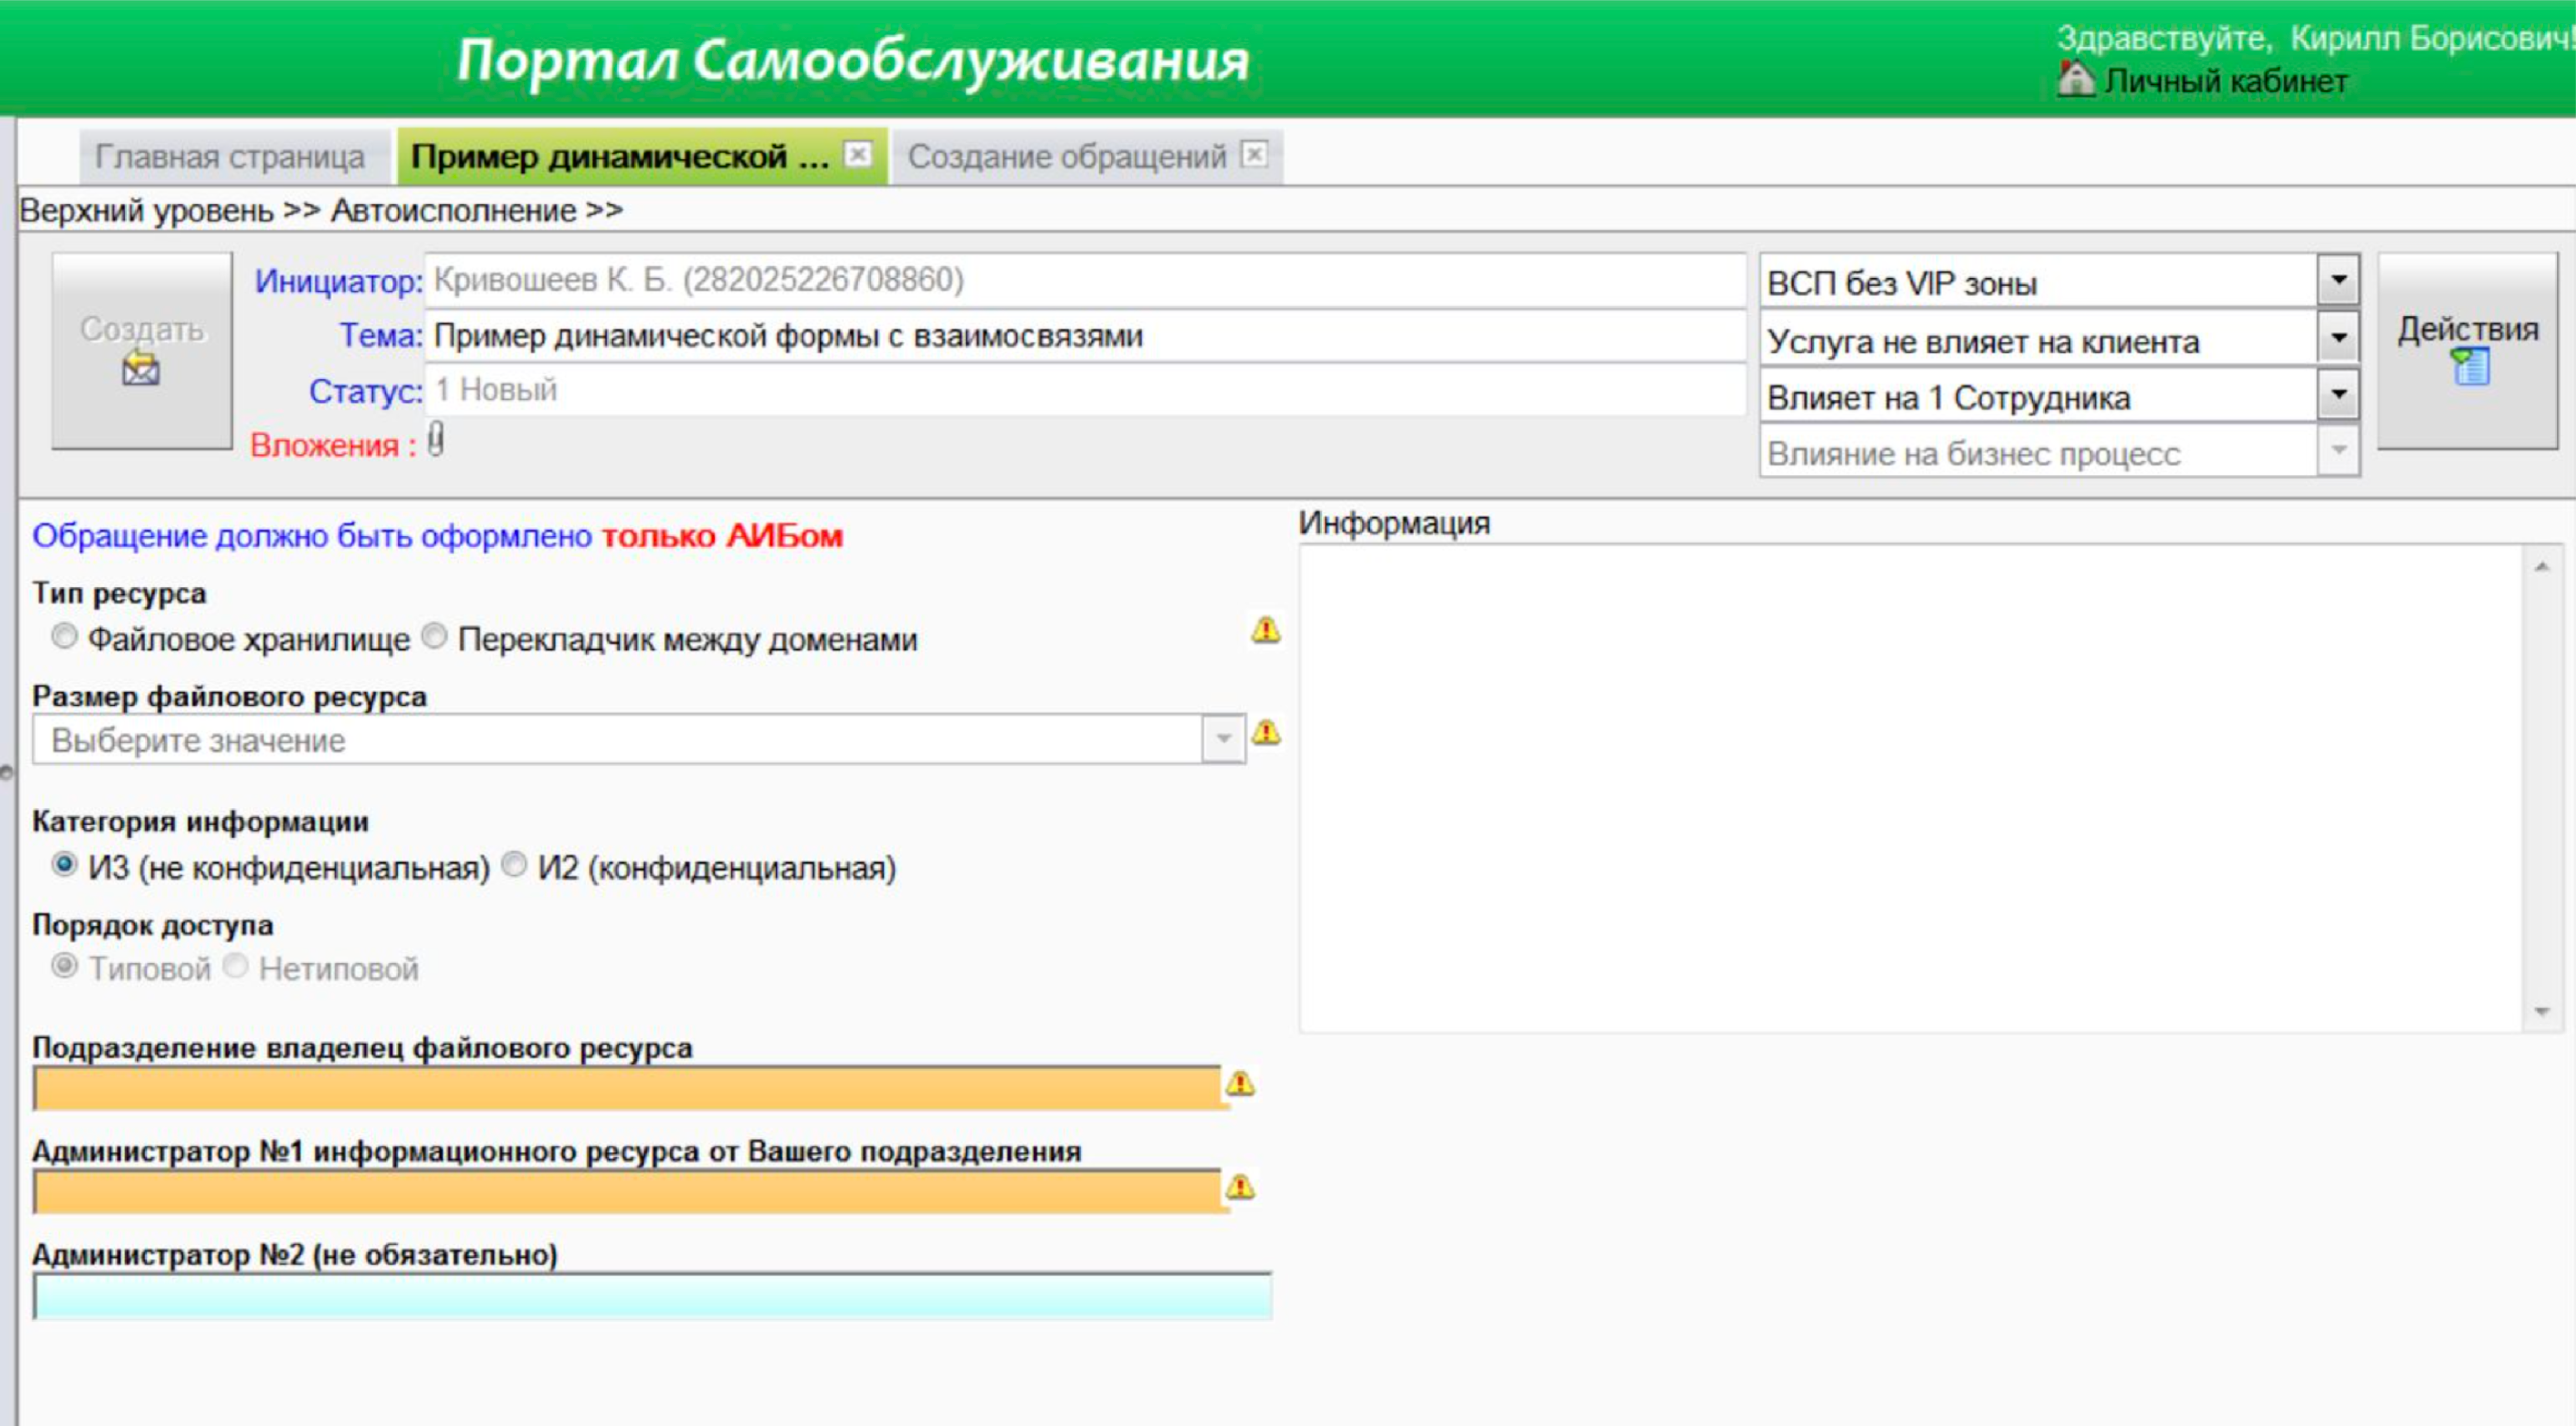
\includegraphics[width=1\textwidth]{portal_2}
	\centering
\end{figure}

Динамический язык однозначно изменил пользовательский опыт в лучшую сторону, но так думали не все. Начальник отдела сервис-менеджеров очень не любил изменения, ведь они чаще всего обозначали, что что-то может сломаться. Стало ясно, что он не согласует внедрение динамического языка на портал, но Кирилла это не остановило. 

Кирилл Борисович просто внедрил язык и уже по факту рассказал, мол, смотрите, как у нас теперь всё здорово работает. 

Какой же поднялся скандал! Что? Зачем? Для Кого? У пользователя и так есть окошко для информации, зачем ему эти поля и чекбоксы, зачем ему вся эта логика? Убрать! Убить! Оторвать! 

“Вырубать, только если топором” — поставил перед фактом Кирилл Борисович, твёрдо веря в то, что поступает правильно.
Как говорится, не все готовы к изменениям и иногда приходится вносить их принудительно.


\section{ДРУГ}

30 января 2014 года Теймур Штернлиб был назначен вице-президентом Сбербанка, и в этой должности планировал реализовать стратегическую программу оптимизации всех обеспечивающих функций банка. 

Вместе с Вячеславом Гавришиным, который на тот момент был бизнес-партнером, они пришли к Кириллу с запросом о портале, в котором пользователи могли бы заказывать услуги не связанные с IT. 

Кириллу в команду дали верстальщика, дизайнера и менеджера. Вчетвером они приступили к работе в феврале 2014. 

Портал нужно было разработать уже к маю того же года, и учитывая что довольно много времени ушло на разработку концепции и дизайн, оставался буквально месяц на написание кода. 

Но если вы прочитали историю выше, то знаете, что Кирилла Борисовича ничего не останавливает, и он справился с задачей. Более того в тоже время поступил заказ от сервис менеджера IT.
Было решено совместить эти 2 портала так, чтобы пользователь не думал о том какую заявку ему надо подать, IT, или нет, у него был единый каталог в котором он мог найти, все что ему необходимо. 

Так и родился ДРУГ, один из крупнейших внутренних порталов для сотрудников Сбербанка.

\begin{figure}[H]
	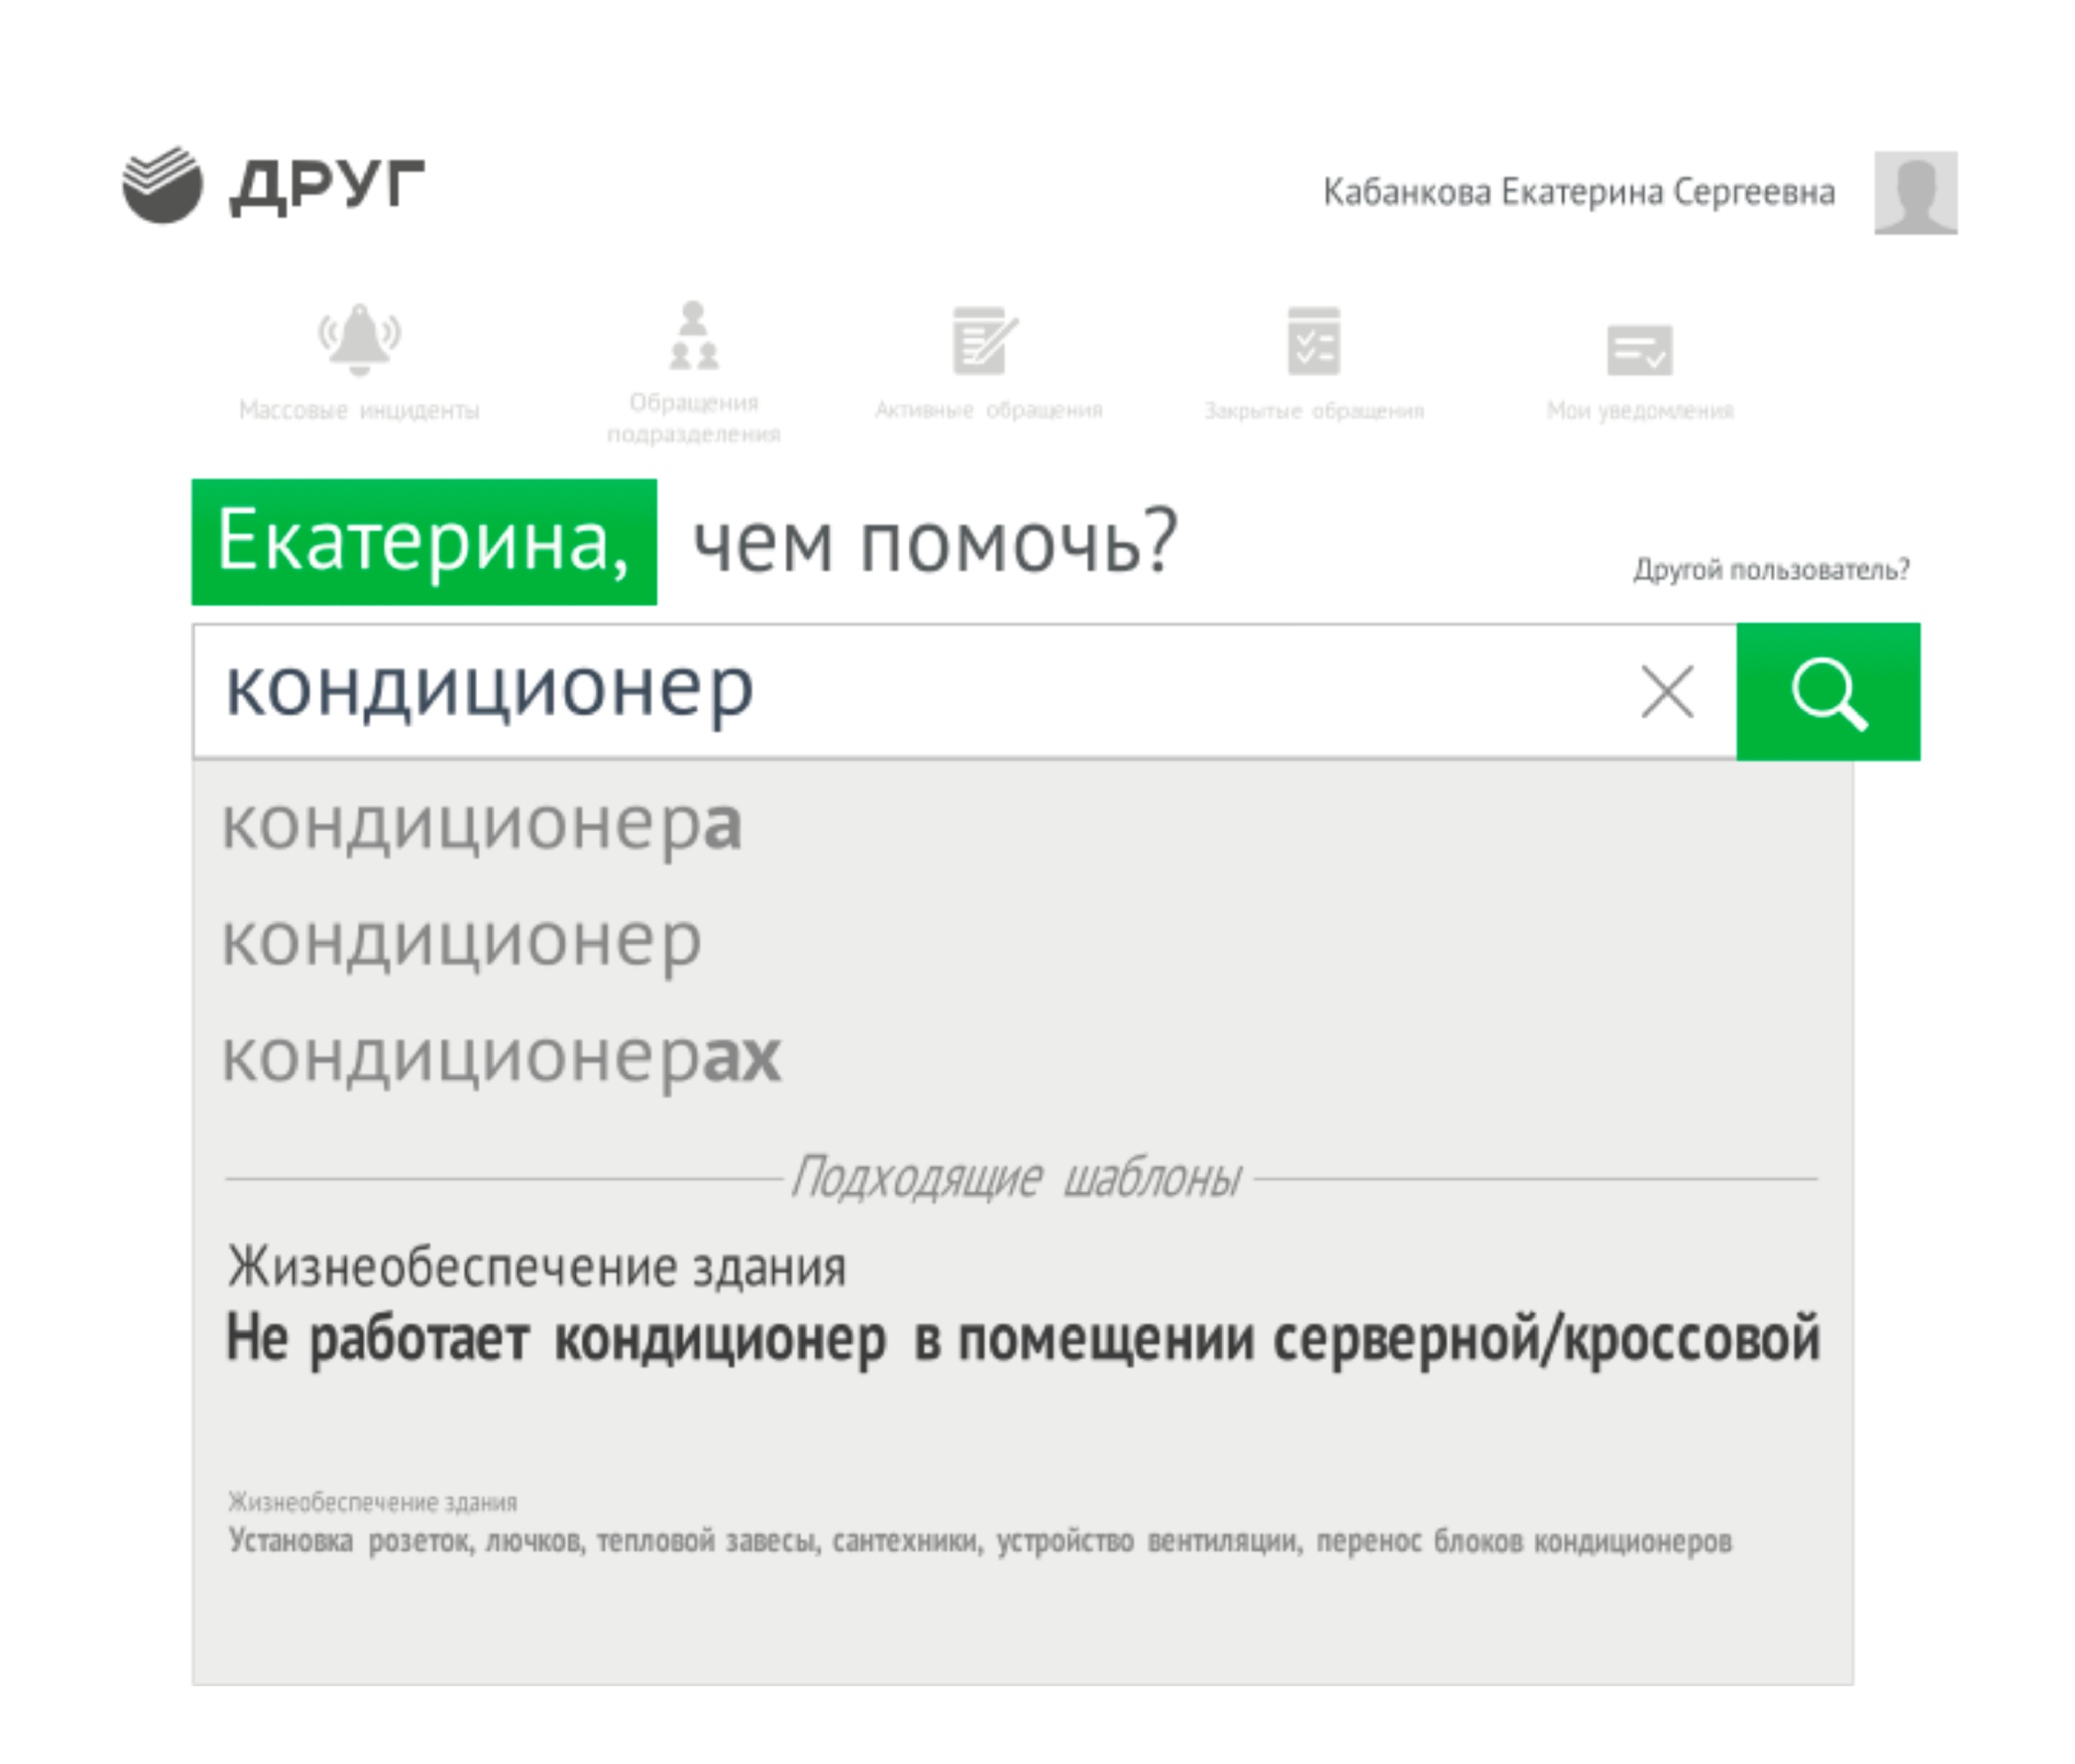
\includegraphics[width=1\textwidth]{friendface}
	\centering
\end{figure}

\section{Команда}

После запуска портала ДРУГ, Теймур принял решение о создании отдельного подразделения, чтобы не было необходимости нанимать кого-либо со стороны и все могли работать вместе и рядом.  

Так наняли сначала 3 человек, и вскоре количество сотрудников в команде дошло до 30. И это была лучшая команда! Кирилл создал вокруг себя очень дружелюбную, благоприятную атмосферу, в которой люди были на первом месте. Все работали ради большой цели и без дополнительных навязанных процессов, команда регулярно выдавала результат.
Можно сказать, что это и был тот самый Agile, к которому сейчас все так стремятся. 

Команда под руководством Кирилла по сей день трудится с горящими глазами, Лицо Друга 1.0 сменилось на Лицо Друга 2.0, а затем на Лицо Друга SE. Мобильное приложение также работает на динамических формах и продолжает развиваться. 

Сам динамический язык также не стоит на месте. Не смотря на то, на сколько круто можно было настраивать и плодить шаблоны, динамический язык достаточно трудно масштабировать, т к по факту его почти никто не знает. Кроме того у него не было единой библиотеки под все платформы, поэтому для того, чтобы добавить какой либо функционал,  это необходимо было сделать отдельно на каждой платформе. 

Теперь же  у динамического языка  появился домик, а точнее dom-core, единая среда выполнения, с поддержкой JavaScript. Это сильно расширило возможности динамических форм, ведь теперь их могут создавать даже студенты, изучающие JavaScript, но это не точно=) 

В общем, благодаря Кириллу, в Сбербанке появилась самая лучшая команда, самый лучший сервис и самый невероятный язык программирования.

Продолжайте читать эту книгу и прикоснитесь к прекрасному. Изучив все главы, вы сможете с легкостью создавать свои шаблоны и команды в 9 листов кода. Удачи!=)
\end{document}
